\chapter{Objectives and Contributions}

\epigraph{As a computer scientist, the most important part of a research is the what, not the how}{\textit{Maria-Esther Vidal}}

\label{chap:objectives}
As discussed in the previous chapters, in our work we focus on the exploitation of declarative mapping rules for the construction of knowledge graphs from heterogeneous data sources. Additionally, in order to evaluate these kinds of systems, we propose and design a set of methodologies and benchmarks. This chapter presents the objectives of our work and identifies our contributions to the current state of the art. We also enumerate the assumptions considered when we started this work, and describe the most relevant hypotheses and restrictions that delimit the scope of this thesis. Figure \ref{fig:objectives_contributions} summarizes the objectives and contributions of this thesis and their relations with the identified restrictions, assumptions and hypothesis.

\section{Objectives}
The principal research question we want to answer in this thesis is: \textit{How can we build more scalable and efficient KG construction engines based on declarative mapping rules, independently of the specification of the mapping language?}. To tackle this open research problem, we identify two main objectives. 
First, our aim is to describe a new generation of KGC engines that use declarative annotations to scale up this process over complex data integration scenarios. The exploitation of these declarative mapping rules and constraints allow the definition of structures and associated operators that enhance virtual and materialized construction of KGs from heterogeneous data sources. The second goal of this thesis is to define objective methodologies to evaluate this new generation of KG construction engines. More in detail, our objective is to create an evaluation framework for materialized and virtual KG construction engines that is general enough to allow the comparison of these systems and also to detect the main limitations of all of them.

The first objective of this thesis (scalable and efficient construction of (virtual) KGs) can be decomposed into the following goals tackling open research problems:

\begin{itemize}
    \item The current heterogeneity in the number of declarative mapping specifications reduces the benefits of this approach for constructing knowledge graphs. Based on the W3C recommendation R2RML~\citep{R2RML}, and with the aim of providing support to other formats beyond relational databases, many new declarative mapping languages have been proposed such as RML~\citep{dimou2014rml}, xR2RML~\citep{michel2015translation}, KR2RML~\citep{slepicka2015kr2rml}, CSVW~\citep{tennison2015model}, or D2RML~\citep{chortaras2018mapping}. When mappings are defined in a specific language, the choice of the KGC engine is more limited. Thus, KG engineers may not benefit from optimizations that are applicable to their use cases but are implemented for another languages. This situation  impacts negatively on the global adoption of these data integration systems in real-world applications of knowledge graphs. Our goal is to provide support for the translation among mapping languages while preserving their features.

    \item The construction of virtual knowledge graphs from heterogeneous data sources (e.g., CSV, JSON, XML or RDB) does not always exhibit good query evaluation performance, nor completeness. The common technique is to use na\"ive SQL data wrappers that hide the complexity of the input sources. However, in order to tackle the advantage of proposed SPARQL-to-SQL optimization techniques~\citep{priyatna2014formalisation,calvanese2017ontop}, well-formed RDB instances are required, including their corresponding domain and integrity constraints. Our goal is to define horizontal solutions that exploit declarative annotations for KGC (i.e., mapping rules and declarative constraints) together with mapping translation techniques to enhance the query evaluation performance and completeness of current SPARQL-to-SQL approaches.

    \item Current approaches for constructing materialized knowledge graphs~\citep{csimcsek2019rocketrml,lefranccois2017sparql} do not scale-up in complex data integration scenarios that are common in the real world (e.g., high rate of duplicates or interoperability issues over the input data sources, high data volume, etc.). The absence of efficient engines that exploit declarative mapping languages to construct materialized knowledge graphs hinders their global and industry adoption over real use cases. Our goal is to develop efficient and horizontal techniques for scaling-up the construction of KG from heterogeneous data sources exploiting declarative KGC annotations.
\end{itemize}

The second goal of this thesis (evaluation methodologies of KGC systems to understand what are their main limits) can be decomposed into the following goals with the associated open research problems:
\begin{itemize}
    \item Current evaluations performed over materialization knowledge graph construction engines are neither representative nor general enough to provide a clear overview of the limitations of the applied techniques. Furthermore, some engines such as RocketRML~\citep{csimcsek2019rocketrml} and SPARQL-Generate~\citep{lefranccois2017sparql} have only been evaluated using their own use cases, datasets and parameters. Our goal is to create an evaluation framework that is general enough and considers as many parameters as possible to allow fair comparisons among KGC engines and the definition of new benchmarks and testbeds including other relevant features .
    \item Virtual knowledge graph construction benchmarks~\citep{lanti2015npd,bizer2009berlin} have mainly focused so far on relational databases, ignoring other types of data sources that are used for KG construction (e.g., CSV, JSON, XML). Hence, they are not enough to test the capabilities of the new generation of engines that are able to run or distribute SPARQL queries over data sources in several formats. Our goal is to define a benchmark for VKGC on a relevant domain allowing the comparison over multiple and heterogeneous virtual KGC engines using a single point, taking into account data sources beyond RDB and relevant parameters that can impact the performance of the engines.
\end{itemize}

\section{Contributions to the State of the Art}
In this work, we aim to provide solutions to the goals and open research problems described in the previous section. The contributions for solving the first research problem are:

\begin{enumerate}
    \item[\textbf{C1.1.}] \textbf{The definition of the concept of \textit{Mapping Translation} and the characterization of its main properties}. We motivate the idea of making the different mapping language specifications interoperable by a new step in a knowledge graph construction workflow, where mappings can be translated to a different specification. Additionally, we define the desirable properties of this concept based on the work of~\citep{hartig2017foundations} and we demonstrate their potential usage over a set of use cases extracted from the literature where it has been successfully applied.
    \item[\textbf{C1.2.}] The \textbf{formalization and application of constraints extracted from mapping rules and metadata over tabular data} to enhance virtual KG construction approaches. Focused on tabular data sources, we extend a typical virtual KG construction workflow adding a set of additional pre-processing steps to handle common issues for querying tabular data sources. Exploiting information from mapping rules and metadata annotations, we are able to efficiently apply integrity and domain constraints, together with a set of new optimization steps, for enhancing both performance and completeness in (virtual) KG construction over tabular sources.
    \item[\textbf{C1.3.}] The exploitation of standard \textbf{declarative mapping rules to automate the generation of functional wrappers} for virtual KG construction. Following best practices on data publication on the web~\citep{bizer2011linked} and with the aim to help knowledge and software engineers to design and implement efficient functional wrappers, we propose a solution that exploits mapping rules for the automatic creation of programmed wrappers. More in detail, we use R2RML mappings and a new interpretation of the SPARQL-to-SQL baseline algorithm presented in~\citep{chebotko2009semantics} for creating programmed and efficient GraphQL wrappers, which allows the translation from GraphQL to SQL queries for obtaining data from relational databases.
    \item[\textbf{C1.4.}] Definition of \textbf{physical operators exploiting information from mapping rules} for constructing materialized KGs at scale. We define a set of data structures aligned with the different types of tasks that a materialization KGC engine has to perform to create the RDF graph. The data structures, together with their corresponding operators, are able to construct materialized KGs in complex data integration scenarios (big data sizes, high rate of duplicates, etc). We demonstrate that our proposal is able to generate KGs at scale in comparison with the state of the art engines. 
    \item[\textbf{C1.5.}] \textbf{Heuristic-based optimizations for functional mappings} (mapping rules with transformation functions) for scaling up the construction of materialized knowledge graphs. Covering the gap of parsing mapping rules that contain ad-hoc transformation functions over the input data sources in an efficient way, we propose a set of mapping and data translation rules to enhance the construction of materialized KGs from this kind of mapping rules.
\end{enumerate}

With regard to the second objective, this work presents new contributions in the following aspects:
\begin{enumerate}
    \item[\textbf{C2.1.}] Definition of a set of \textbf{test cases to evaluate the conformance of KG construction engines in RML}. We extend the R2RML test cases~\citep{R2RML_test_cases} to cover other kinds of data formats and relational databases. Executed over the RML parsers in its corresponding RML implementation report, they give an overview of the current state of the engines in terms of language conformance.
    \item[\textbf{C2.2.}] Identification and experimental evaluation of the \textbf{parameters that affect the behavior of the KGC engines}. We analyze the typical inputs and their corresponding features in a knowledge graph construction workflow and how they can impact the performance and completeness of the process. Additionally, we empirically demonstrate the importance of taking into account these parameters (e.g., join selectivity, data partitioning, duplicate generation) for generating representative benchmarks and testbeds for these engines.
    \item[\textbf{C2.3.}] Design of a complete and \textbf{representative benchmark for evaluating virtual KGC engines}, based on open data from the transport domain. We created Madrid-GTFS-Bench, a comprehensive benchmark for virtual knowledge graph construction, which considers multiple data formats and different data scales. Several engines are evaluated with a single benchmark so as to assess the current status of virtual knowledge graph access.
\end{enumerate}

Chapter \ref{chapter:mappig-translation} describes the mapping translation concept and its properties.Chapter \ref{chapter:evaluation} describes the GTFS-Madrid-Bench, a virtual knowledge graph construction benchmark in the transport domain, aligned with the second objective. In the same Chapter, two evaluation methods for testing mapping compliance and performance during the contruction of materialized KG are presented. Chapter \ref{chapter:virtual} provides the solutions to enhance virtual knowledge graph access over heterogeneous data exploiting the mapping translation concept. Finally, Chapter \ref{chapter:construction} presents two approaches for scaling up the construction of materialized KGs. 

\section{Assumptions}
Our work is based on the assumptions listed below. These assumptions provide a background to facilitate the comprehension of the decision taken during the development of this thesis.
\begin{enumerate}[label=\textbf{A{\arabic*}}]
    \item Mapping rules and metadata descriptions are declarative and follow W3C standards (or their extensions). Although the contributions proposed in the thesis may be generalized to any kind of mapping rules and metadata descriptions, we assume that these annotations are defined following best practices for describing content on the web of data, hence, using W3C standards. 
    \item The target schema (ontology) for integrating the source data is available and is implemented in OWL. We also assume that in any of the data integration systems ($DIS$) defined in this thesis, the target model used for integrating the input sources has been already created, and it is modeled using the Web Ontology Language (OWL).
    \item Mapping rules and metadata descriptions are available. In the same manner as the ontology, the rules that provide the relations between target and source schemes and metadata that describe the content of the source input data are available. Therefore, we assume that the $DIS$ presented in the thesis are complete and no user interaction is needed.
    \item Data are represented in formats that are not RDF. The input data sources that have to be integrated in a $DIS$ are described in formats such as RDB, CSV, XML or JSON, but we assume that none of the datasets will be described following RDF.
    \item Datasets are static, not streams. We assume that the input data sources are static, although they can have a short update time (e.g., 5 minutes), the proposals of this thesis do not provide support for data streams.
\end{enumerate}

\section{Hypothesis}
After the identification of the assumptions, we can describe the research hypothesis of this thesis. They cover the general characteristics of the contributions.
\begin{enumerate}[label=\textbf{H{\arabic*}}]
    \item It is possible to translate declarative mapping rules among different specifications allowing practitioners to have the possibility of selecting a wider set of engines to construct their KG. Our hypothesis here is that mapping translation techniques can be used to enhance multiple features of a KG construction workflow such as mapping rules generation, maintainability, optimization techniques, etc.
    \item The exploitation of mapping rules and metadata descriptions for data constraint extraction and its application can enhance the performance, access and completeness of current virtual knowledge graph construction systems. This can be performed by extending the current virtual KG construction workflow, including a set of efficient additional steps for the application of the extracted constraints over the input sources. 
    \item A benchmark based on \texttt{de-facto} standard models for publishing transport data on the web is able to stress and provide a full overview of the current state of different types of virtual knowledge graph construction engines. The intrinsic features of these data models, a well defined target ontology, and a set of relevant queries covering SPARQL 1.1 features are able to define a representative benchmark that addresses the strengths and limitations of virtual KG construction engines and applied techniques.
    \item Using the information from the input mapping rules, physical data structures and their corresponding operators can be defined for scaling up the construction of materialized KGs from heterogeneous data sources. These structures can handle complex data integration environments where a large number of joins among sources and a high rate of duplicates have an impact over the performance of the KG construction. 
    \item Optimizations for processing functional mapping rules can be applied to scale up the construction of materialized knowledge graphs. The application of efficient techniques for pre-processing transformation functions during a KG construction process, together with mapping and data translation rules, can deal with complex data integration systems. 
    
\end{enumerate}

\section{Restrictions}
Finally, there is a set of restrictions that describe the limitations and define the future work objectives. The restrictions are:

\begin{enumerate}[label=\textbf{R{\arabic*}}]
    \item Input data sources must be located in the same physical place as the one where the knowledge graph construction process is run. We do not consider network latencies for data transference or other similar parameters that may have an impact over a process of constructing a KG. 
    \item We do not have to consider data protection nor access restrictions. We assume that there are no limitations to access any of the input data sources of the $DIS$. The datasets are openly available through the web together with a license that allows its use.
    \item The size of datasets is defined in terms of Gigabytes. We assume that each single input data source will be no bigger than 100Gb.
    \item Our proposal does not make use of the capabilities of SPARQL-to-SQL engines. We do not exploit the specific optimizations that each engine applies, we are only aware about the importance of indexes and integrity database constraints for the effectiveness of their translation process.
    \item Our proposal does not make use of the features of the transformation functions performed over the input data sources. Therefore, we are not aware about  the transformation functions being bijective or not, which can have an impact over query translation techniques.  
\end{enumerate}



\begin{figure}[!t]
\centering
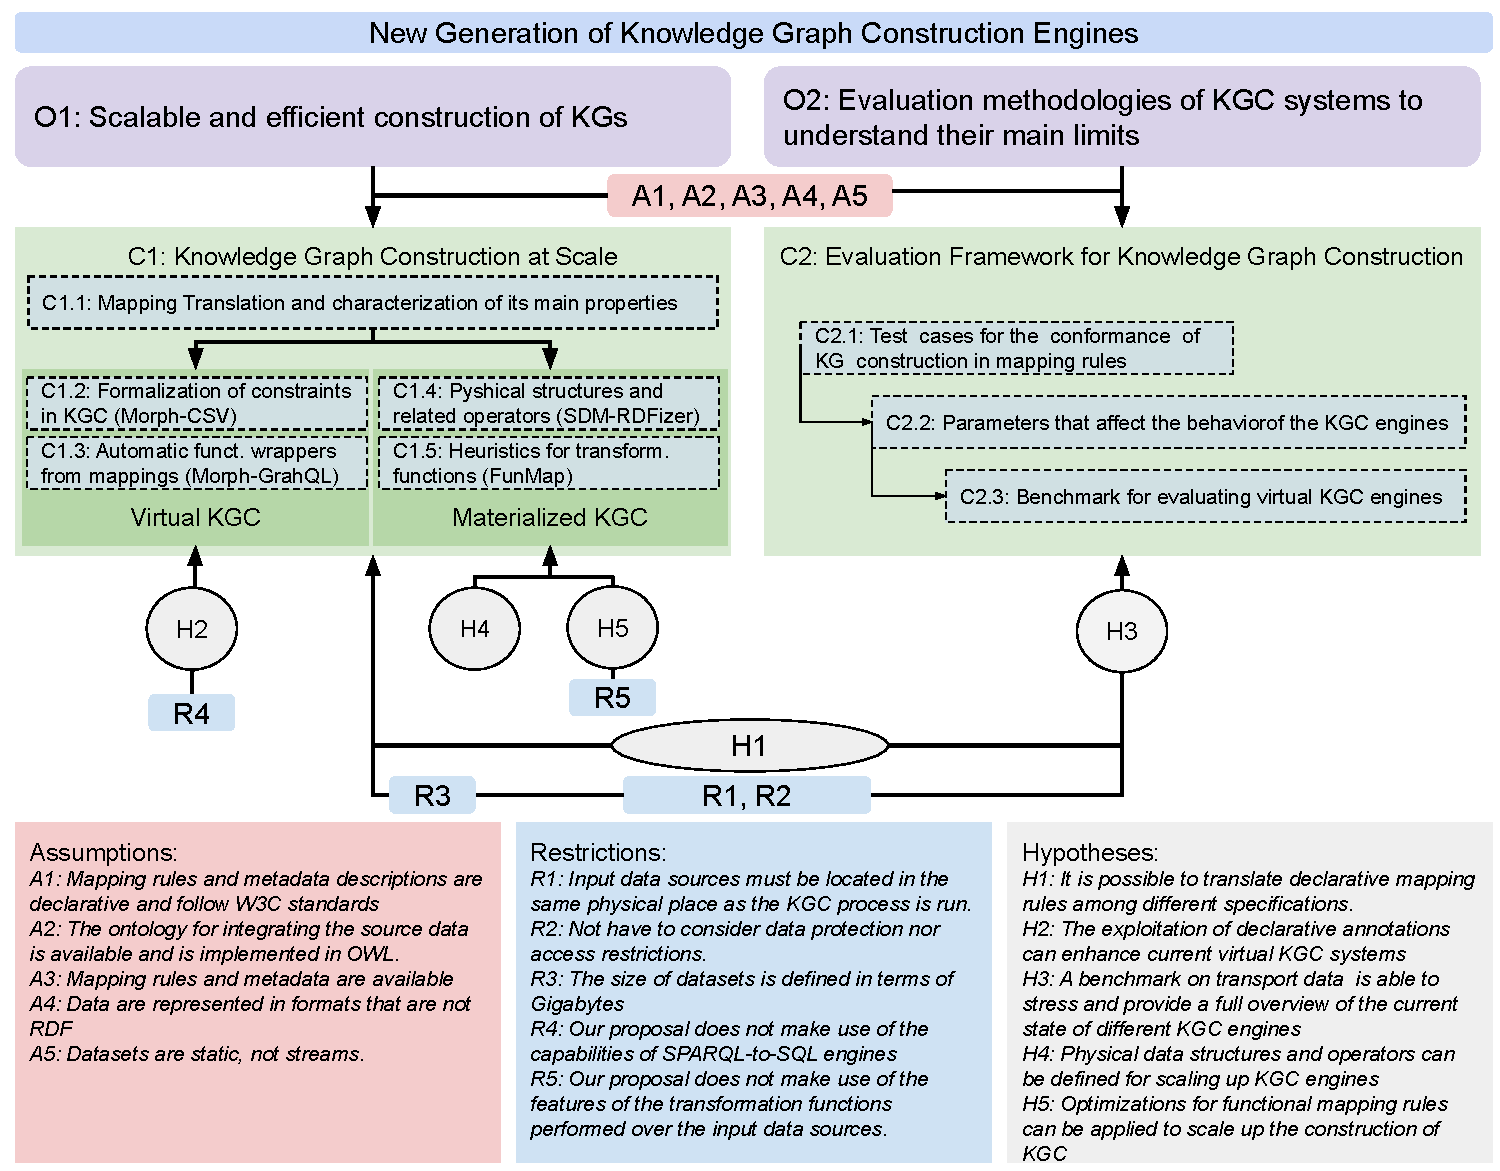
\includegraphics[angle=90,width=1\textwidth]{figures/summarize contributions.pdf}
\caption[Relations of the contributions of the thesis]{Contributions, Hypotheses, Assumptions, Restrictions and Objectives of the thesis with their relations}
\label{fig:objectives_contributions}
\end{figure}